\chapter{Introduction}\label{intro}

	When gravitational waves were first detected in September 2015, the first question was, "Is it real?". The next was, "How do we get more?".
	
	The Laser Interferometer Gravitational-Wave Observatory (LIGO), was built with the purpose of detecting the ripples in space-time caused by astrophysical events to understand the complexities hidden in the cosmos.  In 2011, the advanced version of the LIGO detectors were installed and commissioned which detected the first signals from colliding black holes \cite{DetectionPaper}.  During the writing of this thesis, the detectors had hardware replaced in order to mitigate noise from scattered light and new optics which reduced the losses from absorption.
	
	The first chapter of this thesis serves as an introduction to gravitational waves and their affect on a simple interferometer. The second chapter will describe the modern detectors and their dominating noise sources.  Chapters 3-6 will be focused on experimental wavefront control for the current generation of detectors and beyond.

	\section{Gravitational Waves}\label{gravitational waves}
	In 1915, Albert Einstein published his theory of general relativity \cite{einstein}, which contains the most complete description of gravity to date.  This theory has stood the test of time and scrutiny by correctly predicting the perihelion of mercury \cite{Einstein_GR}, the bending of light from massive objects \cite{DysonEddington}, and the loss of energy from gravitational radiation \cite{HulseTaylor}. The seminal equation in this theory, called the Einstein Field Equation is
	
	\begin{equation} \label{einstein}
	G_{\mu \nu} = 8 \pi T_{\mu \nu}
	\end{equation}
	
	which is a set of 10 coupled second-order differential equations that are nonlinear and fully describes the interaction between space-time and mass-energy. Equation \ref{einstein} is difficult to solve except in situations where specific approximations allow a user to find exact solutions such as spherical symmetry \cite{carroll_2003} \cite{schutz_2009}. In areas where the curvature is close to flat,  the weak field approximation can be applied and the metric is described as	
	
	\begin{equation} \label{weak}
	g_{\mu \nu}  \approxeq \eta_{\mu \nu} + h_{\mu \nu}
	\end{equation}
	
	where $\eta_{\mu \nu}$ is the metric of flat spacetime and $|h_{\mu \nu}| \ll 1$ is the perturbation due to a gravitational field.	By plugging in equation \ref{weak} into \ref{einstein} and using empty space we obtain the familiar wave equation
	
	\begin{equation} \label{wave}
	\Big(\nabla^2 - \frac{1}{c^2} \pdv[2]{t} \Big) h_{\mu \nu}  = 0
	\end{equation}

	which has a plane-wave solution of the form $h_{\mu \nu} = A_{\mu \nu} e^{ik_{\nu} x^{\nu}}$. Using the gauge constraint $h^{\mu \nu}_{,\nu} = 0$, it follows that $A_{\mu \nu} k^{\mu} = 0$ which means that the gravitational wave amplitude is orthogonal to the propagation vector. Further imposing transverse-traceless gauge and assuming that the wave is traveling in the $x^3$ direction, it can be shown that the complex amplitude has physical significance expressed in the matrix
	
	\begin{equation} \label{gwamp}
	A_{\mu \nu} = 
	\begin{pmatrix}
			0 &    0   &  0      & 0 
		 \\ 0 & A_{xx} &  A_{yx} & 0
		 \\ 0 & A_{xy} & -A_{xx} & 0
		 \\ 0 &    0   &  0      & 0
	\end{pmatrix}
	\end{equation}

	Oftentimes, the four non-zero components of equation \ref{gwamp} can be categorized into two distinct polarizations: plus and cross where $h_{+} = A_{xx} = -A_{yy}$ and $h_{\cross} = A_{xy} = A_{yx}$ .
 
	Consider the four-velocity, $U^{\alpha}$, in the transverse traceless gauge where the coordinate itself is attached the particles and incorporates any small wiggles that would shake the coordinates.  Of course, any free particles will follow the geodesic equation
	\begin{equation}\label{geodesic}
	\nabla U^{\alpha} = \frac{\text{d}}{\text{d} \tau} U^{\alpha} + \Gamma^{\alpha}_{\mu \nu} U^{\mu} U^{\nu} = 0
	\end{equation}	
	where $\Gamma^{\alpha}_{\mu \nu} = \frac{1}{2} g^{\gamma \alpha}(g_{\gamma \mu, \nu} + g_{\gamma \nu,\mu} - g_{\mu \nu, \gamma} )$ are the famous Christoffel symbols.
	By evaluating the first term of the acceleration in equation \ref{geodesic},
	\begin{equation}\label{accel}
	\bigg(\frac{\text{d}U^{\alpha}}{\text{d}\tau}\bigg)_0 = -\Gamma^{\alpha}_{00} 
	\\ = \frac{1}{2} \eta_{\mu \nu} (h_{\beta 0, 0} + h_{0 \beta, 0} + h_{0 0, \beta} )
	\end{equation}
	
	\begin{figure}[ht]
		\centering
		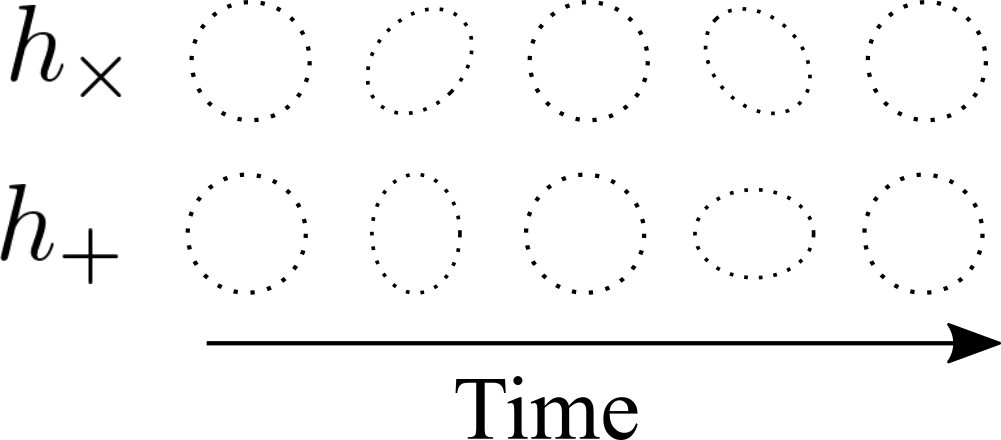
\includegraphics[width=.4 \textwidth]{../Figures/GW_Particles.png}
		\caption[A ring of free floating particles being stretched and squeezed by a passing gravitational wave.]  
		{\textbf{Effects of a gravitational wave.} A ring of free floating particles will be stretched and squeezed by a passing gravitational wave, the two pictures represent the plus and cross polarizations.}
		\label{fig:gwparticles}
	\end{figure}
	
	However, comparing equation \ref{gwamp} and equation \ref{accel}, it is clear that if the particle is initially at rest, then a moment later it is still at rest! The term "at rest" is actually used liberally here since the coordinate system varies along with the gravitational wave.  To understand the physical interpretation of equation \ref{gwamp}, imagine the gravitational wave propagating towards a ring of free floating particles in space.  The spacetime will be modulated in a squeezed and stretched motion as shown in Figure \ref{fig:gwparticles}.  
	
	Alternatively, one can ask if a gravitational wave passed by a pair of particles separated by length $L$, what would be the effect on the distance between two points \cite{SaulsonStretch}?  The proper distance is defined as

	\begin{equation}\label{propdist}
	\delta l
	= \int{g_{\mu \nu} dx^{\mu} dx^{\nu}} \\
	= \int_{0}^{L}{g_{xx} {d}x}\\
	\approx |g_{xx}(x=0)|^{1/2}\\
	\approx [ 1 + \frac{1}{2} h_{xx}(x=0)] L
	\end{equation} 
	
	which shows us two very important points about the nature of gravitational waves.  Firstly, the effect is very small since the length variation, $h_{xx}$, is a small perturbation on flat space-time.  Secondly, the effect is proportional to the initial separation between the particles. This means a detector which is large will have a better chance to measure these small effects, an important point that drove the design of the Laser Interferometer Gravitational-Wave Interferometer (LIGO).
	
	\section{Measuring Gravitational Waves with Light}\label{measuringGWs}
	Even with the theoretical formulation of gravitational waves resolved by the 1970s \cite{PiraniPhysicalSignificance}, developing a method of detecting gravitational waves with ground-based instruments was still a controversial topic among scientists in the field \cite{CollinsGravity}.  During the famous Chapel Hill Conference in 1957, which included some of the great minds of the era such as Wheeler, Schwinger, and Feynman, the experimental search for gravitational waves began to take hold.  One thought experiment that was proposed by Feynmann \cite{SmootBrief} where he considered a bead sliding on a string with friction as a gravitational wave passes by.  As the bead slides back and forth due to the wave described by equation \ref{propdist}, there will be some heat dissipated which means the gravitational wave must carry some energy.
	
	There is still the issue of an incredible amount of accuracy required to measure the strain from even the most dense astrophysical objects. The earliest attempts at detecting these small signals were famously done by Joseph Weber \cite{Weber} using large resonant bars and piezoelectric transducers to extract the energy from gravitational waves at the resonant frequencies of the bars.  However, these bars are limited by thermal noise and could only detect GWs in very narrow frequency bands. 
	
	With the development of lasers in the 1960s which created coherent and spatially confined light that could propagate long distances.  As light travels in space, it picks up an important quality called $\textit{phase}$ as a function of distance.  Interferometers are devices that measure small displacements by using a laser that is split by a partially transmitting mirror, which allows 50$\%$ of the light to get reflected and 50$\%$ to be transmitted.  Each of the beams travel down the arms and reflect off of mirrors and return to the beamsplitter.  Upon reaching the optic, the two beams recombine and by the principle of superposition  the electromagnetic waves will add linearly at the output port (or antisymmetric port), Figure \ref{fig:simple_michelson}.  The laser beams will gather phase as they propagate down each individual arm, and when recombining, the intensity of the light will be proportional to the phase differences between each beam.  This will correspond to a differential length that is described by
	\begin{equation}
	L_{-} = l_{x} - l_{y}
	\end{equation}
	
	\begin{figure}[ht]
		\centering
		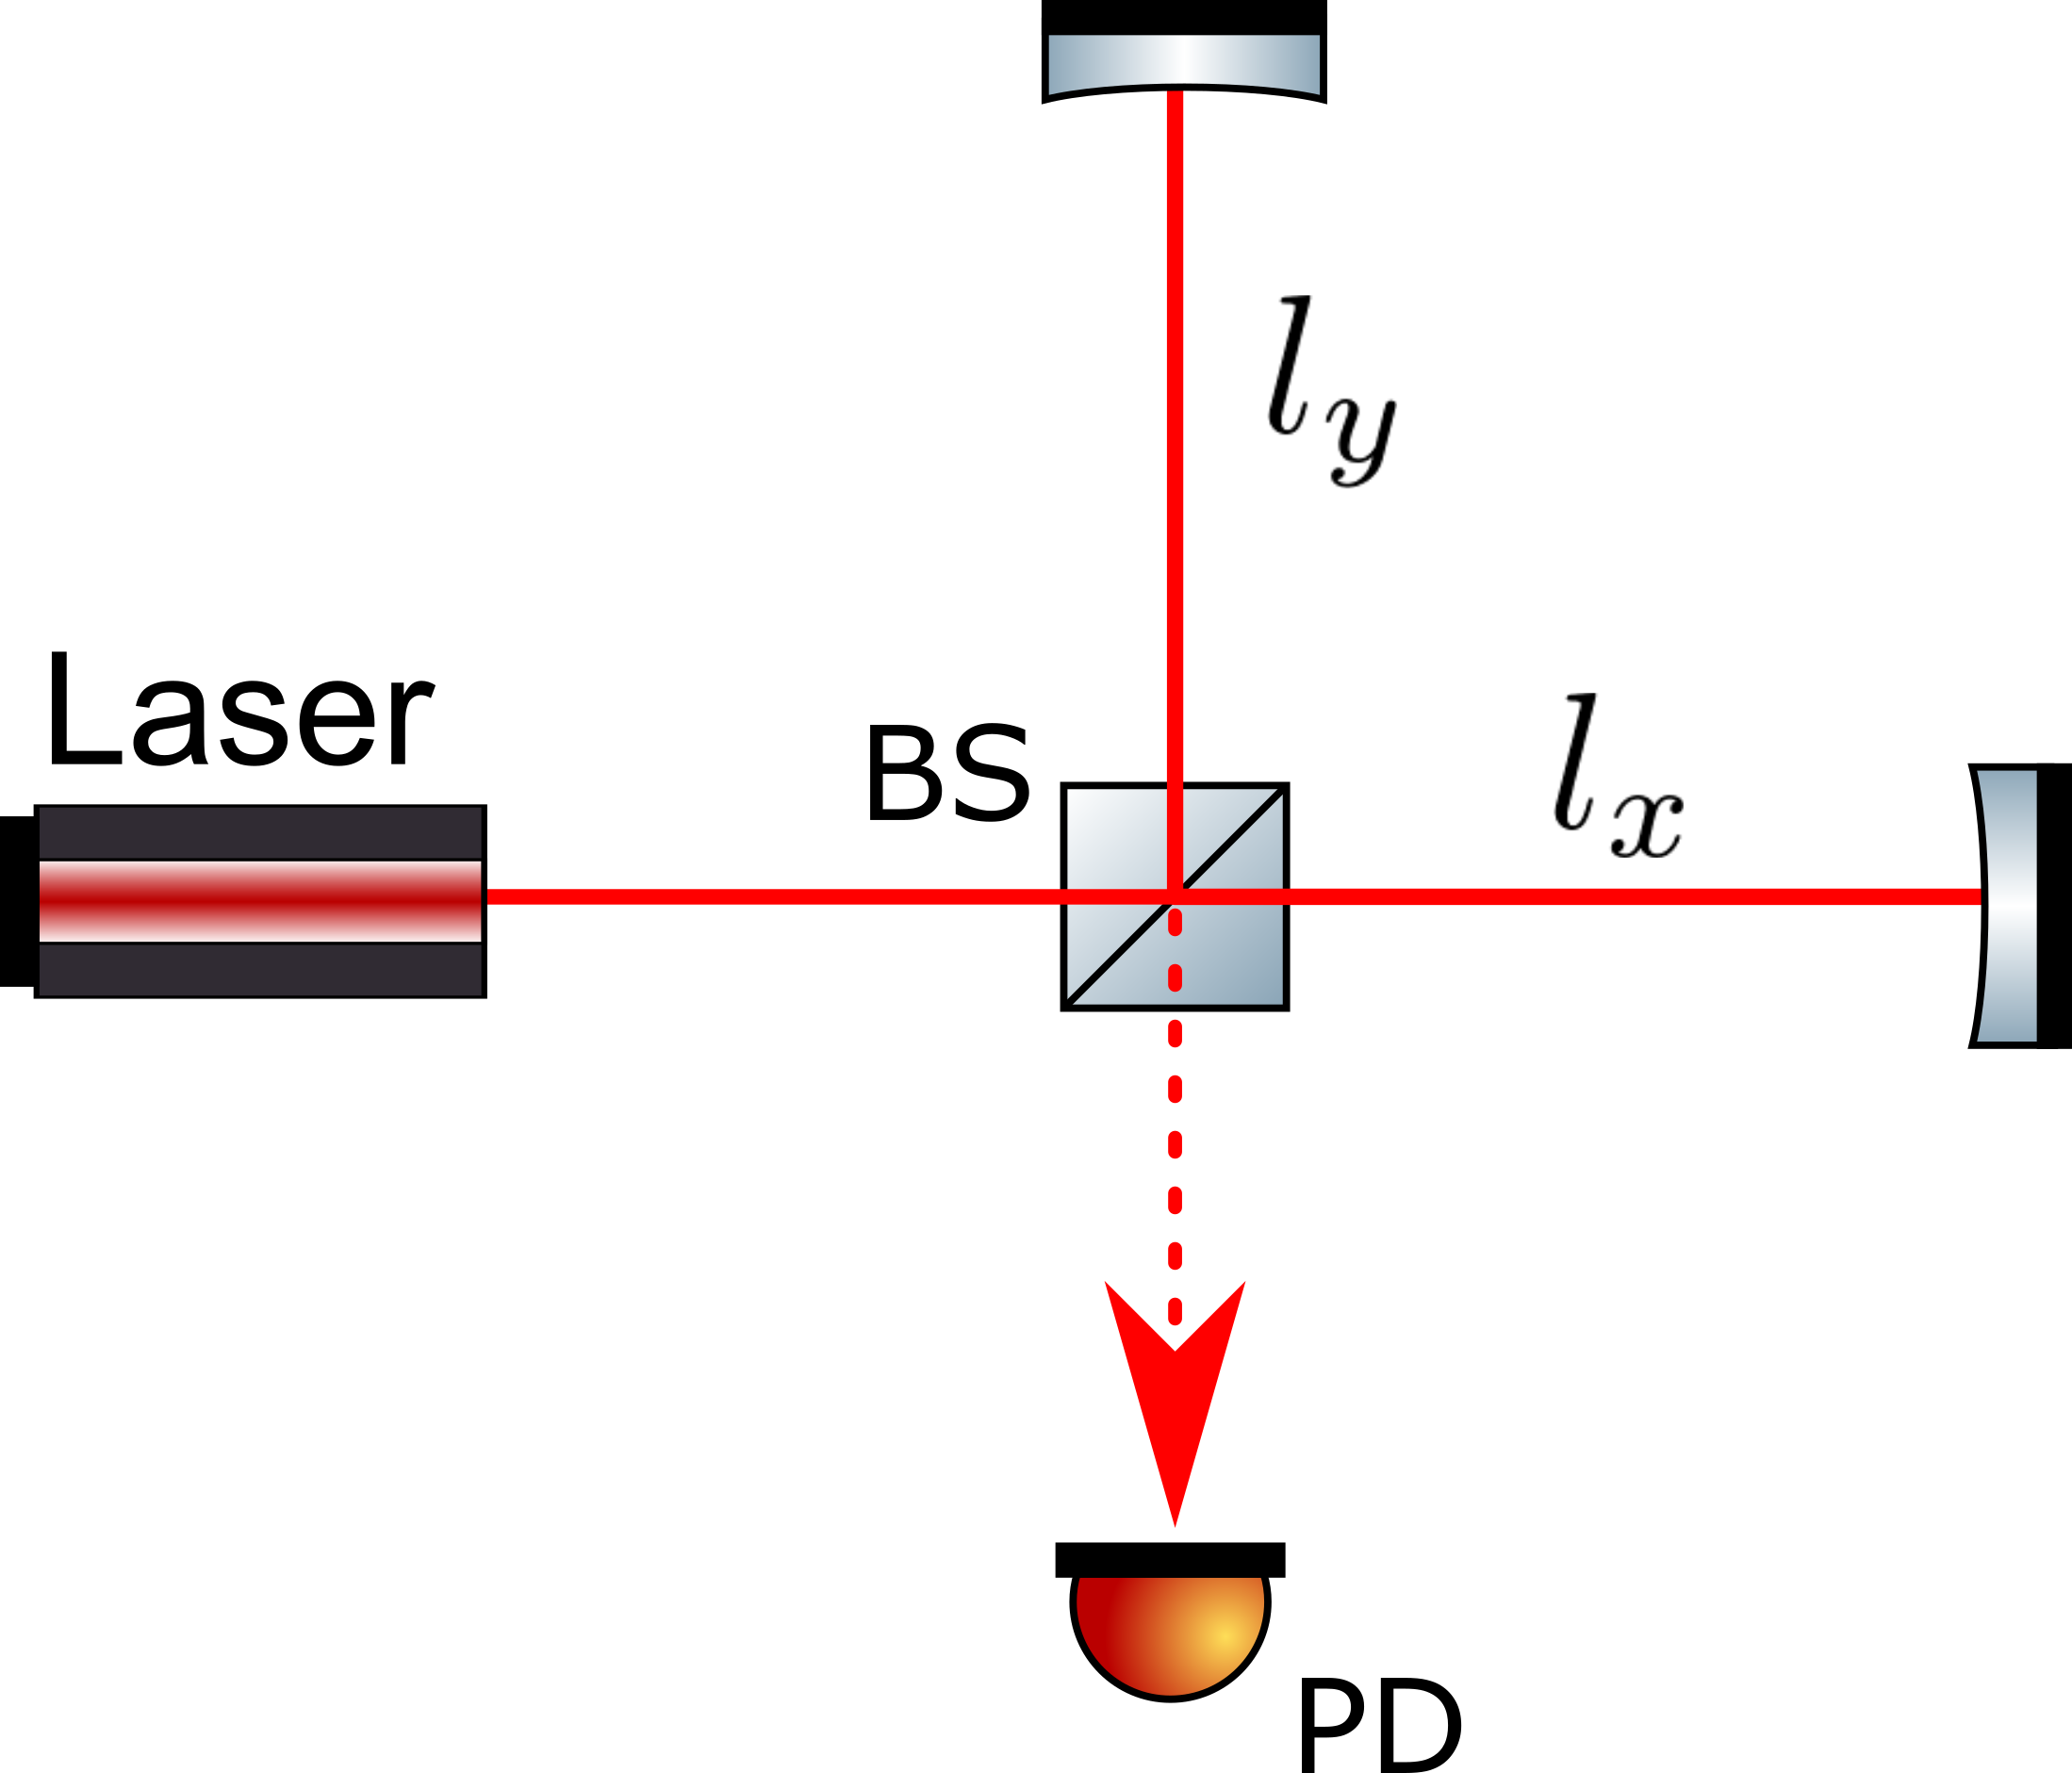
\includegraphics[width=.45 \textwidth]{../Figures/SimpleMichelson.png}
		\caption[A Michelson Interferometer.]  
		{\textbf{A Michelson Interferometer.} A laser is split between with a partially transmitting optic called a beamsplitter (BS), then propagate down each arm to reflect off mirrors, sometimes called test masses (TM).  The beams return to the beamsplitter and recombine, photodetectors are placed at the antisymmetric port (AS).   }
		\label{fig:simple_michelson}
	\end{figure}
	As shown in equation \ref{propdist}, the effect of gravitational waves on the proper length between two free falling objects is proportional to the initial separation.  From Figure \ref{fig:gwparticles}, it is intuitively clear that interferometry would be an ideal technique to detect signals from a gravitational wave.  However, one can explicitly derive an interferometer's response to a GW from an astrophysical object.
	
	First, denote the detector's coordinates using $\hat{x}$ and $\hat{y}$ to co-align with the interferometer arms respectively such that the $\hat{z}$ axis points directly towards the zenith. Now consider a gravitational wave source arbitrarily located in the sky with respect to the Earth with the axis of propagation pointed in the $\hat{z}'$ direction.  Using the well known Euler angles, a relation from the detector frame to the source frame with coordinates $\{\hat{x}',\hat{y}',\hat{z}'\}$ can be seen in Figure \ref{fig:euler}. 
	
	If a gravitational wave at the source has emitted GWs with plus and cross polarizations as denoted by equation \ref{gwamp}, then the detector time series can be regarded as \cite{S6sensitivity} \cite{Finn:1995}
	\begin{equation}
	h(t) = F_{+}(\theta,\phi,\psi) \, h_{+}(t) + F_{\times}(\theta,\phi,\psi) \, h_{\cross}(t)
	\end{equation}
	where $F_{+}(\theta,\phi,\psi)$ and $F_{\cross}(\theta,\phi,\psi$ are the antenna pattern functions that project the gravitational wave amplitudes onto the detector frame shown in Figure.
	
	\begin{equation}\label{Fplus}
	F_{+}(\theta,\phi,\psi) = -\frac{1}{2}[1+\text{cos}^2(\theta)] \text{cos}(2\phi) \text{cos}(2\psi) - \text{cos}(\theta) \text{sin}(2\phi) \text{sin}(2\psi)
	\end{equation}
	\begin{equation}\label{Fcross}
	F_{\cross}(\theta,\phi,\psi) = + \frac{1}{2}[1+\text{cos}^2(\theta)] \text{sin}(2\phi) \text{cos}(2\psi) - \text{cos}(\theta) \text{sin}(2\phi) \text{sin}(2\psi)
	\end{equation}
	\begin{figure}[ht]
		\centering
		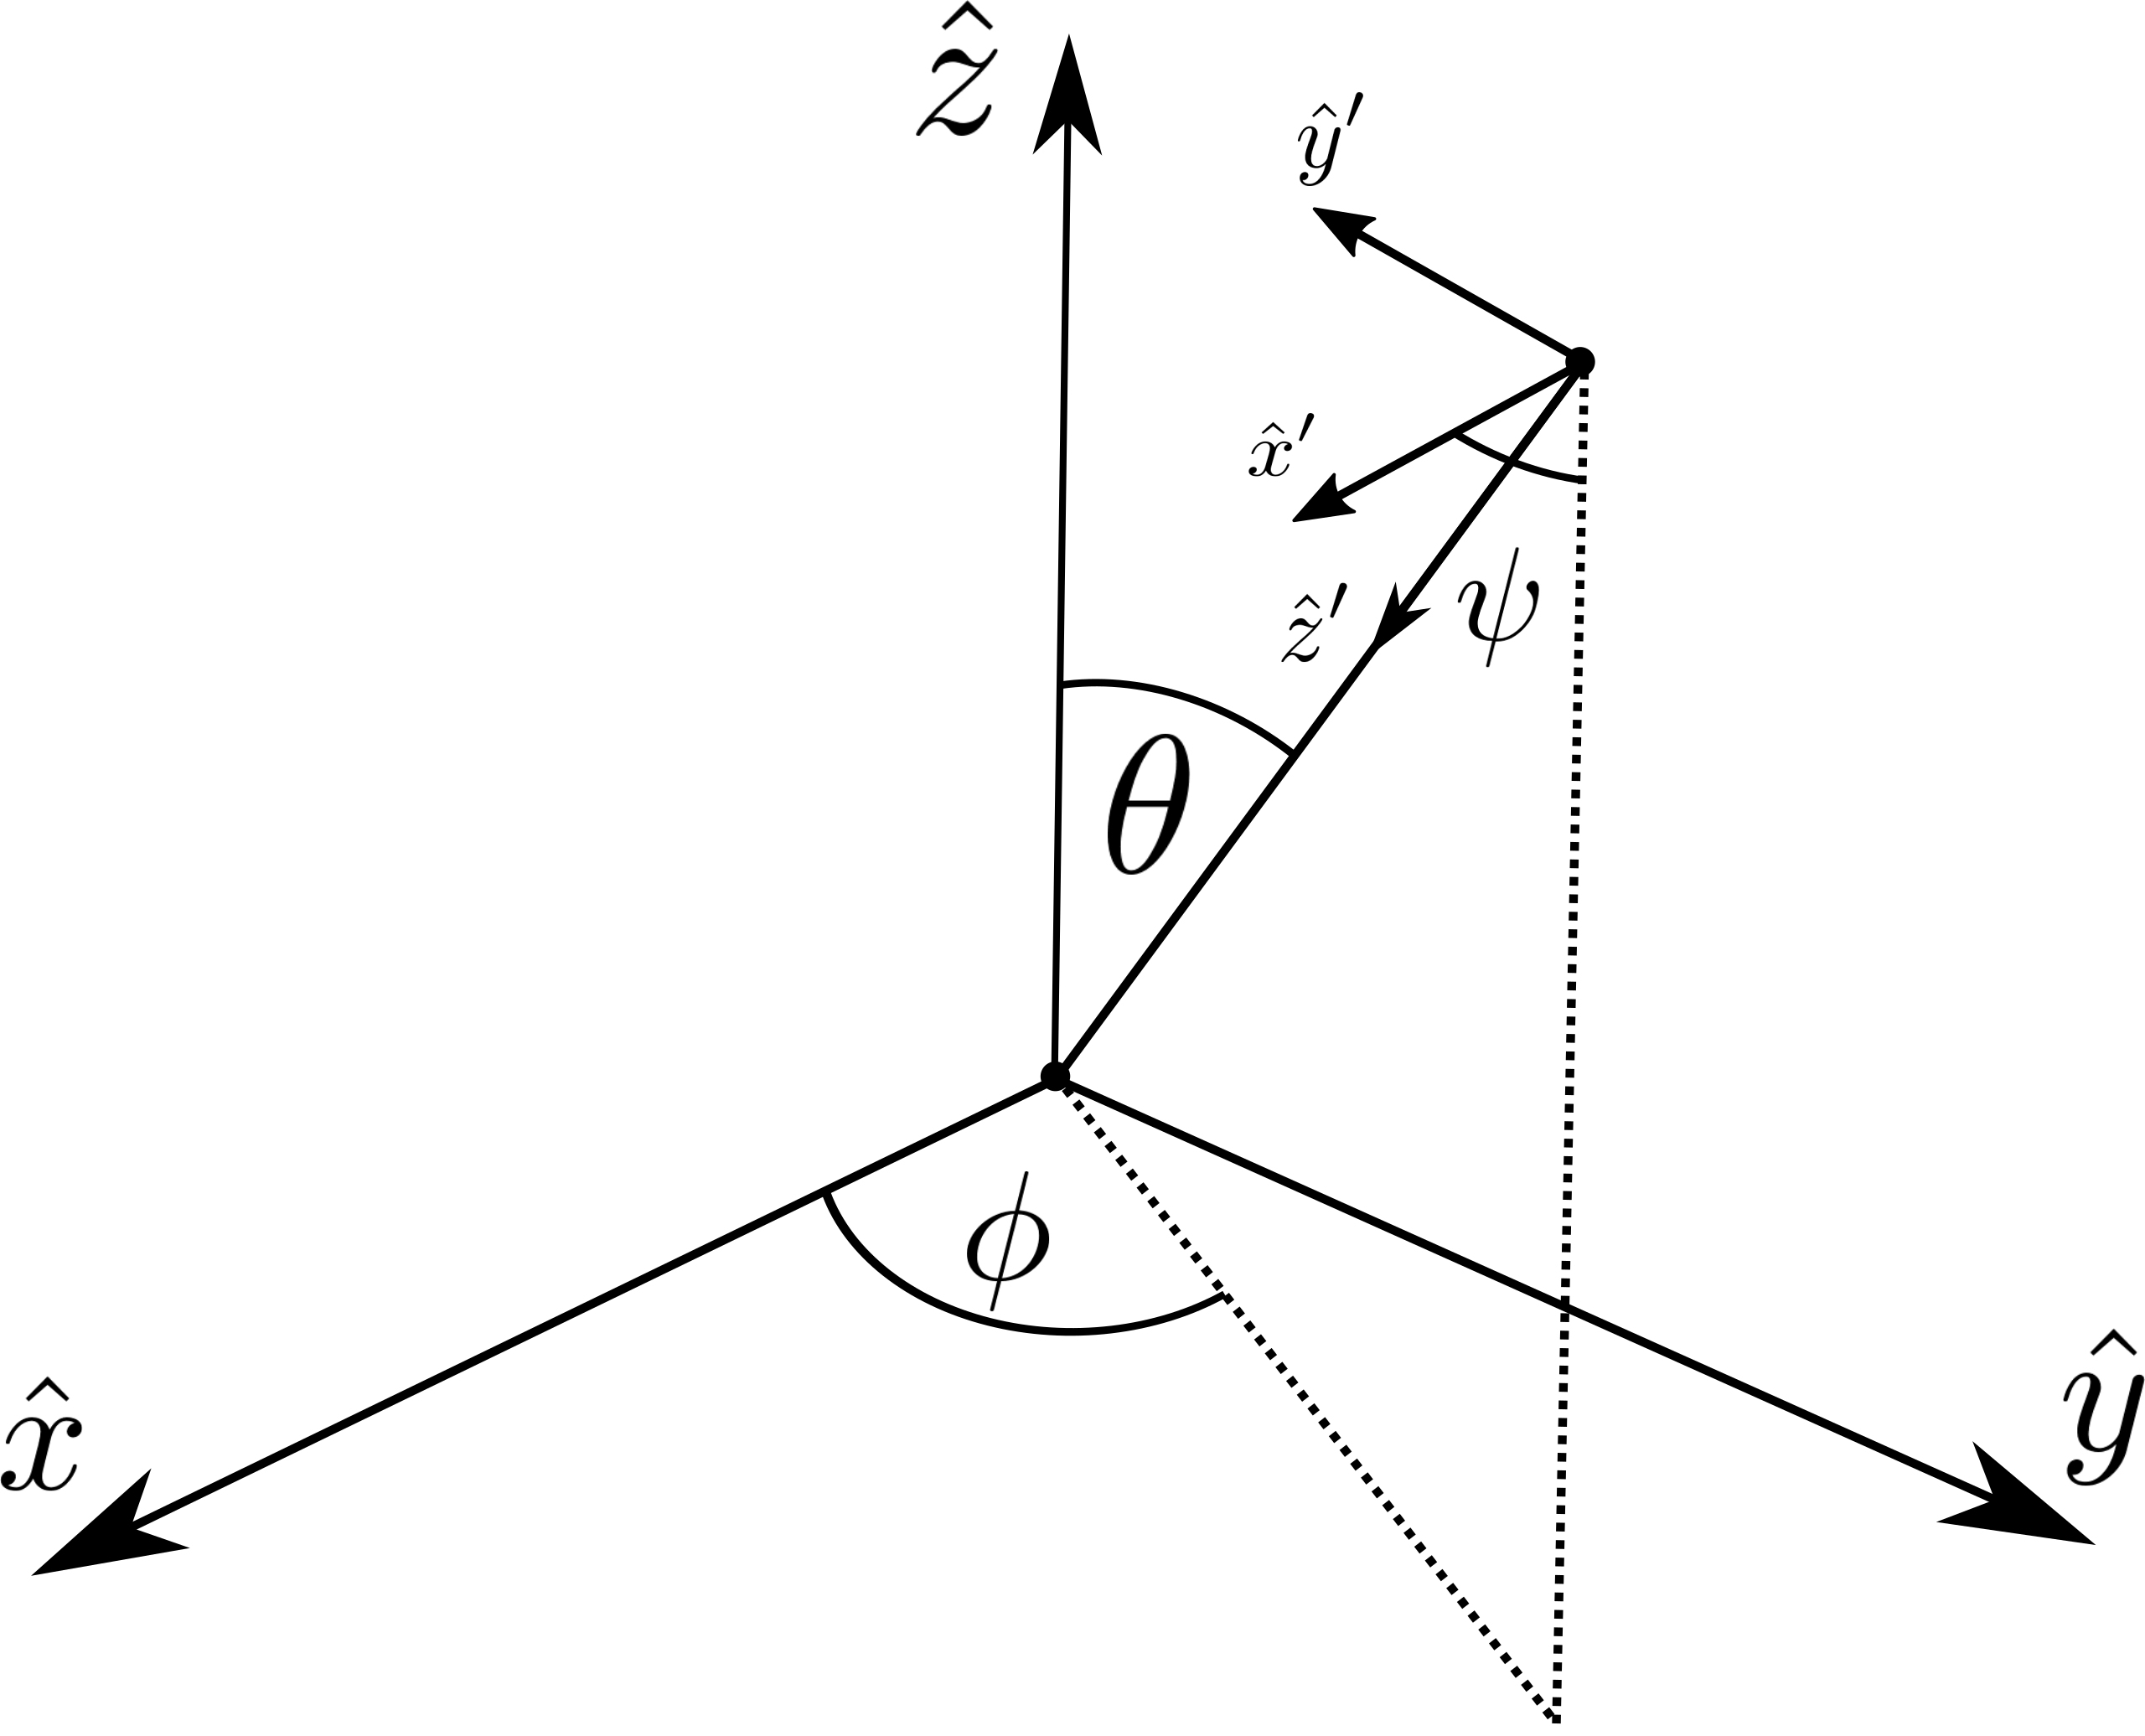
\includegraphics[width=.45 \textwidth]{../Figures/EulerAngles.png}
		\caption[Detector to radiation frame.]  
		{\textbf{Euler angles of gravitational radiation to the detector frame.}  The $\hat{x}$ and $\hat{y}$ coordinates line up with the arms of the interferometer whereas $\hat{z'}$ corresponds to the gravitational wave pointing. }
		\label{fig:euler}
	\end{figure}
	If the gravitational wave is located directly above the interferometer such that $\theta = 0$ and setting $\psi=0$, then the magnitude of the antenna pattern is equal to unity.  Furthermore, by rotating about the $\phi$ angle such that the detector arms align with the plus polarization, the null geodesic equation (ie the path of a photon) in the interferometer frame becomes 
	
	\begin{equation}
	ds^2 = g_{\mu\nu}dx^{\mu} dx^{\nu} = -dt^2 + [1+h_{+}]  dx^2 + [1-h_{+}]  dy^2 + dz^2 = 0
	\end{equation}
	
	Now, if the photon is traveling along the x-arm, this means that $dy^2 = dz^2 = 0$ and the metric equation transforms to
	
	\begin{equation}
	\frac{dt}{dx} = \sqrt{ 1+h_{+} } \approx 1+\frac{1}{2} h_{+} 
	\end{equation}
	
	The amount of time required for the photon to reach the x-end mirror (starting at $t=0$) is equal to
	
	\begin{equation}\label{pathlength}
	t_1 = \int_{0}^{L_{x}} [1+\frac{1}{2}  h_{+}(x) ] \text{d}x
	\end{equation}
	
	where $L_x$ is the total length of the x-arm.  Upon returning to the beamsplitter, the photon's total time of flight for the x and y arms are, respectively,
	
	\begin{equation}
	t_2 = 2 L_x + \frac{1}{2} \int_{0}^{L_x} \bigg[  h_{+}(x) +  h_{+}(x + L_x)  \bigg] \text{d}x
	\end{equation}
	\begin{equation}
	t'_{2}= 2 L_y - \frac{1}{2} \int_{0}^{L_y} \bigg[  h_{+}(y) +  h_{+}(y + L_y)  \bigg] \text{d}y
	\end{equation}
	
	If the gravitational wave period is much longer than the time of flight, then $h_{+}$ does not change much during the measurement, which means $h_{+}(\eta_i) \approx h_{+}(\eta_i + L_{\eta_i}) \approx constant$.  By subtracting the flight times of the photons for each arm and setting $L = L_x = L_y$, the difference is proportional to the gravitational wave perturbation multiplied by the sum of arm lengths (with a factor of $c$ to get the units right),
	
	\begin{equation}
	\Delta t = t_2 - t'_{2} = \frac{2L}{c} h_{+}
	\end{equation}
	By recasting the expression for time of flight in terms of the phase picked up laser light as it travels through space, the differential phase shift is
	\begin{equation}\label{diffphase}
	\Delta \Phi = \Phi(t_{2}) - \Phi(t'_{2}) = \frac{4 \pi}{\lambda} \, h_{+} \, L
	\end{equation}
	
	The equation above is simple, however, it only works for gravitational wave signals that are not frequency dependent and it assumes that the path length can be arbitrarily long. Both points are actually not true \cite{Saulson} but we can alleviate these discrepancies by considering a gravitational wave signal of the form $h(t) = h_0 \, e^{i 2 \pi f_{GW} t}$  and repeating the calculation between equations \ref{pathlength} and \ref{diffphase}:
	
	\begin{equation}\label{gwsinc}
	\Delta \Phi (t) = h(t) \; \tau_{RT} \; \frac{2 \pi c}{\lambda} \; \text{sinc}(f_{GW} \tau_{RT}) e^{i \pi f_{GW} \tau_{RT}}
	\end{equation}
	
	where $\tau_{RT} = 2L/c$.  The response for a detector has null points from the sinc function that is dependent on the gravitational wave frequency and the round trip time constant.  Which means that the instrument cannot be arbitrarily long, however, this point is not concerning because it is too expensive and difficult to make a terrestrial detector of this size.  On the other hand, space-based detectors such as the LISA project will have to account for this effect.  Figure \ref{fig:sincgw} compares the response of an interferometer with 4 km arms versus 100 km, there is larger low frequency response for the longer detector but has large dips when approaching the kilohertz regime where solar mass compact binaries tend to merge.
	
	\begin{figure}[ht]
		\centering
		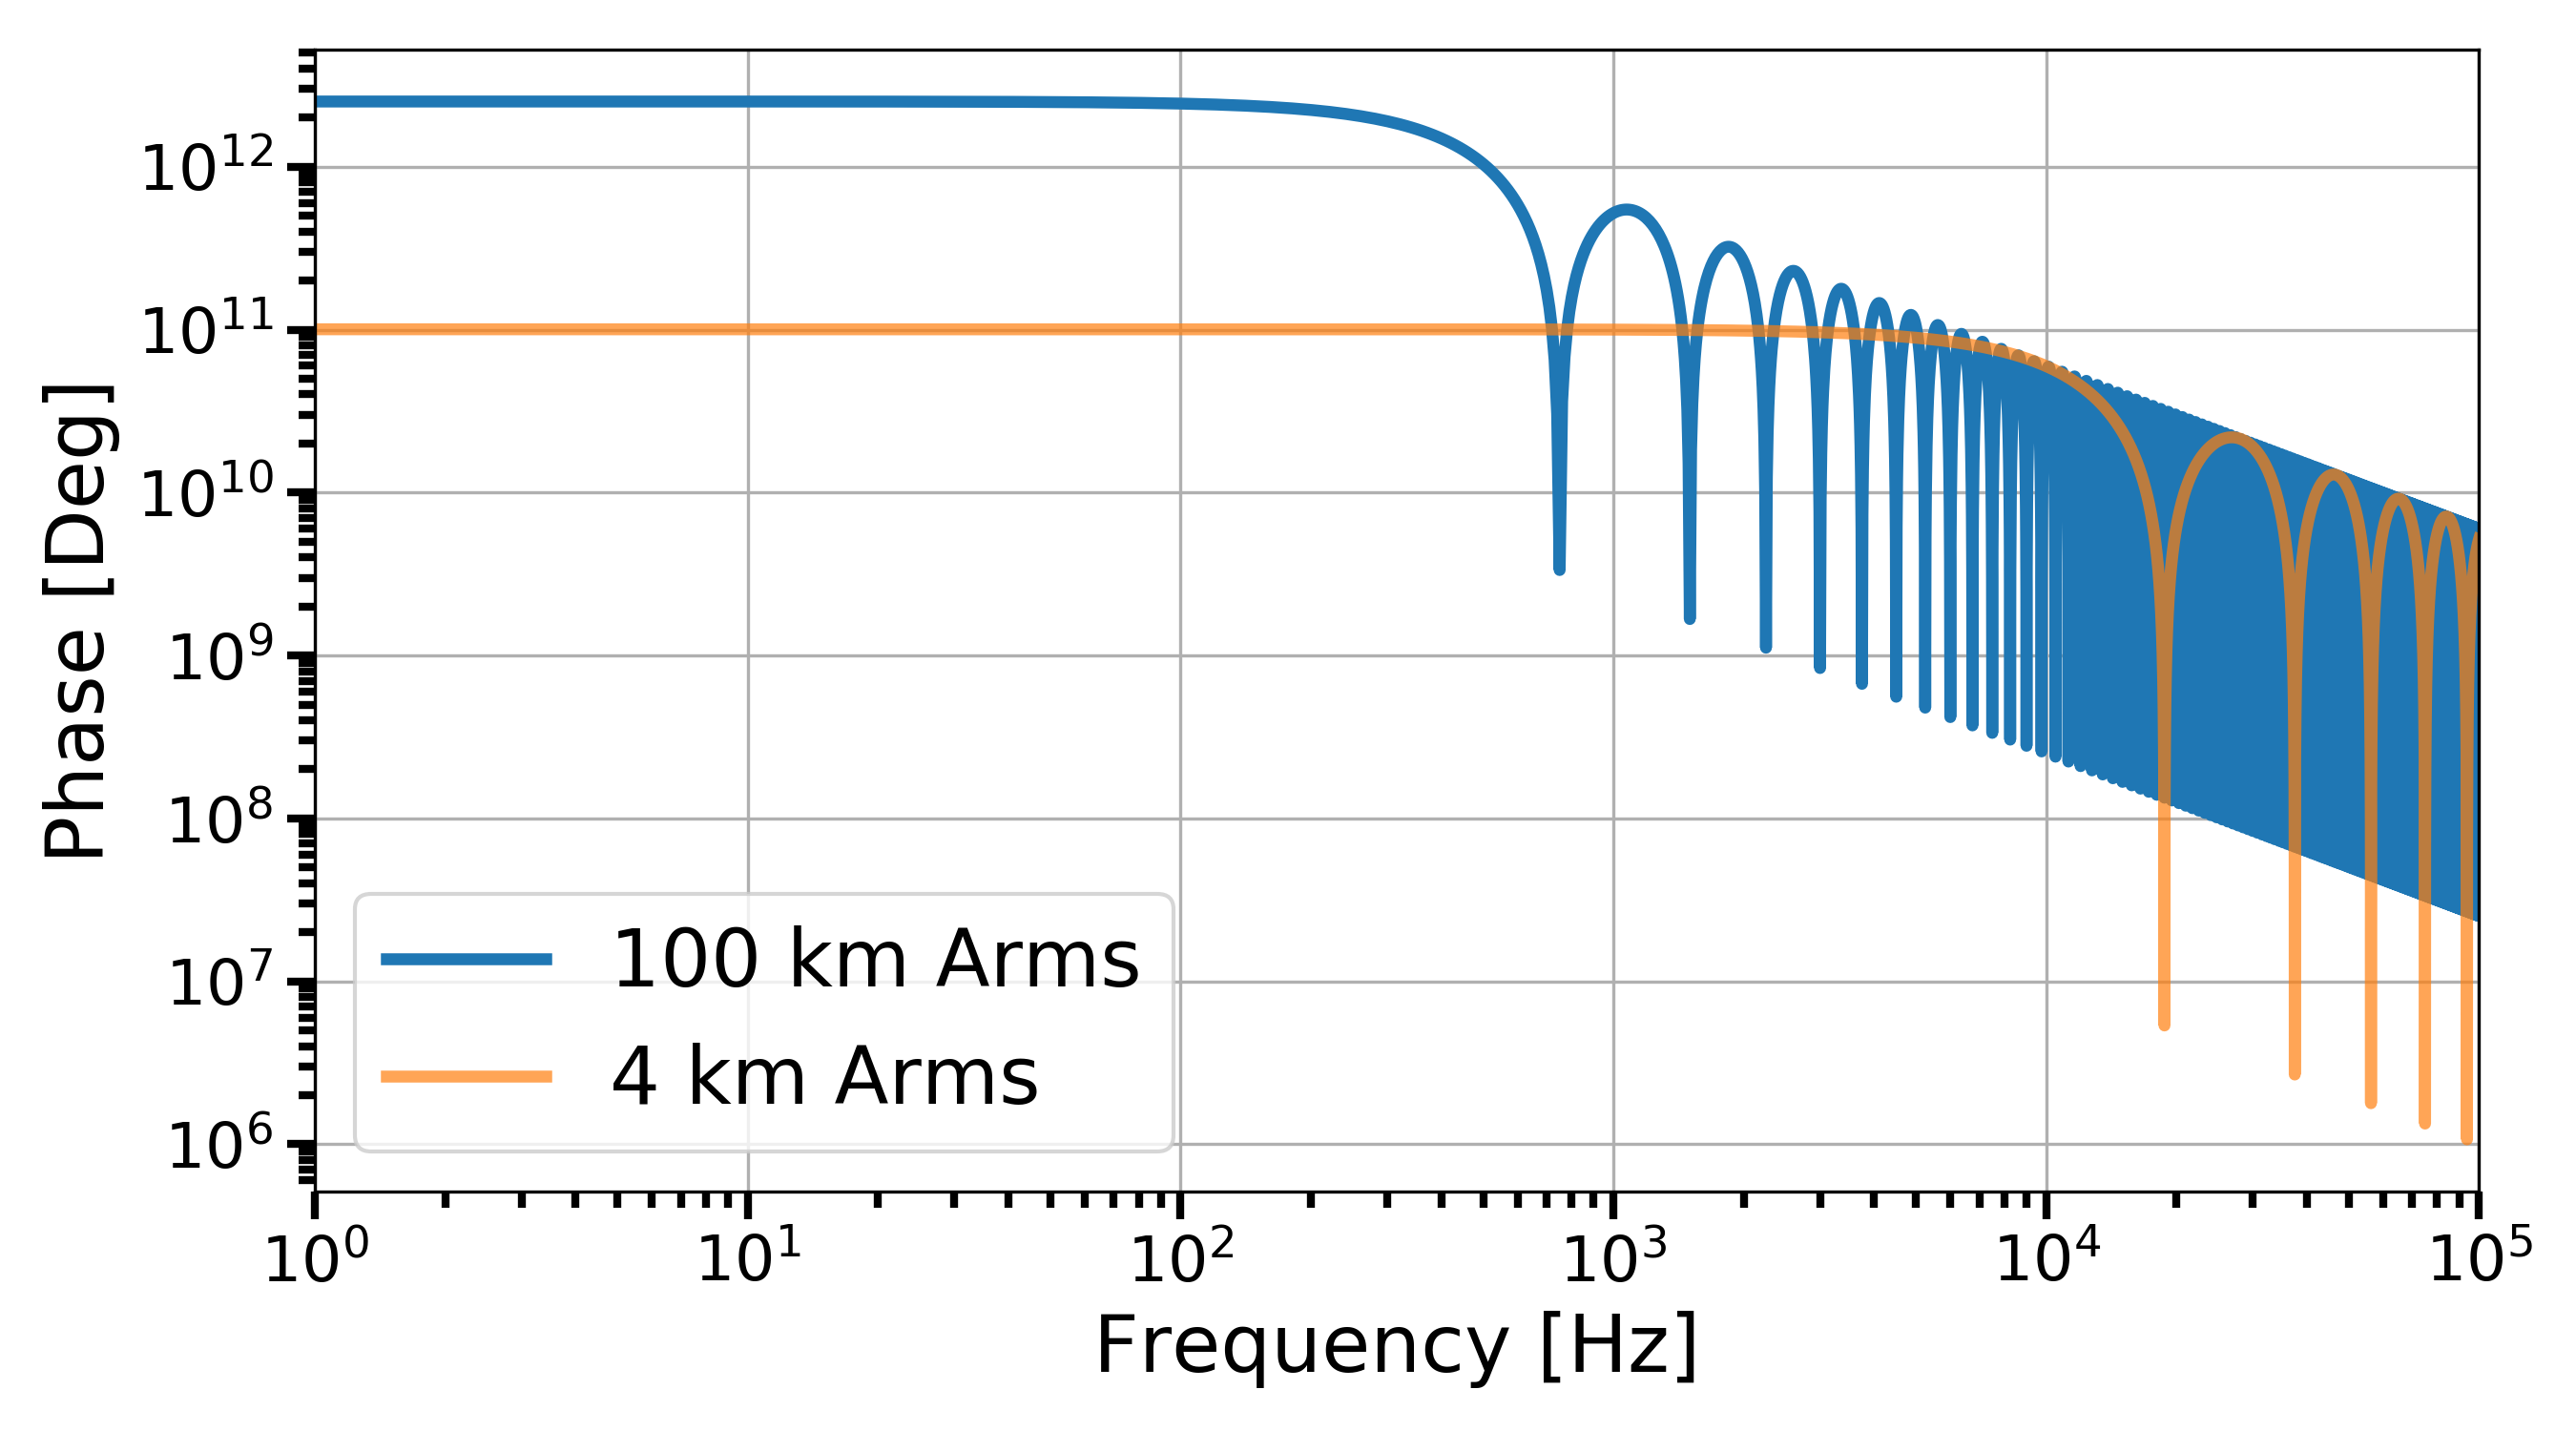
\includegraphics[width=.7 \textwidth]{../Figures/SincGW.png}
		\caption[The phase response of an interferometer to a gravitational wave.]  
		{\textbf{The phase response of an interferometer to a gravitational wave.} The x-axis is in GW frequency and the y-axis is the accumulated phase}
		\label{fig:sincgw}
	\end{figure}
	Laying out the response to gravitational waves is one thing but practically measuring $\Delta \Phi$ to detect astrophysical objects requires much more complex systems, so building modern detector is explained in section \ref{LIGOInstrument}.

	\section{Detection of Gravitational Waves}\label{detectgw}
	The purpose of LIGO is to observe gravitational waves emanating from astrophysical objects \cite{NSFproposal}, so it is natural to wonder how well a single detector can probe the universe.  It is worthwhile to explicitly derive the inspiral horizon distance, which is how far a single detector can detect a binary system comprised of two equal mass compact objects optimally oriented in the sky relative to the detector.  Signal-to-noise (SNR) is the comparison of foreground triggers to the background noise, which can be expressed as
	\begin{equation}\label{SNR}
	\rho = 2 \int_{-\infty}^{\infty} \frac{ \tilde{s}(f) \tilde{s}^*(f) }{S_n(f)}
	\end{equation}
	where ${S_n(f)}$ is the one-sided average power spectral density of the detector noise and $\tilde{s}(f)$ is the Fourier transform of the detectors' response to a gravitational-wave signal.
	
	Consider two dense objects which are approximated by points sources with mass $m_1$ and $m_2$ spiraling around each other.  They are separated by a distance $R$ such that the quadrupole equation from \ref{weak} still holds (i.e. flat space-time with small perturbations). The detector response, in units of strain, to the gravitational waves emitted by this type of source is \cite{Finn:1995},
	\begin{equation}\label{inspiralsignal}
	s(t) = \frac{\mathcal{M}}{d_L} \Theta(\theta,\phi,\psi,i) [\pi f(t) \mathcal{M}]^{2/3} \cos[\Phi(t) + constant]
	\end{equation}
	where 
	\begin{subequations}
		\begin{equation}\label{chirp}
	\mathcal{M} = (1+z) \frac{(m_1 m_2)^{3/5}}{(m_1 + m_2)^{1/5}}
		\end{equation}
		\begin{equation}\label{orient}
	\Theta(\theta,\phi,\psi,i) \&= 2 \sqrt{	[F_{+}(\theta,\phi,\psi) (1+\cos^2(i)) ]^2 + [2 F_{\cross} \cos(i)]^2 }
		\end{equation}
	\end{subequations}
	and $F_{+}$ and $F_{\cross}$ are the antenna response of the interferometer in equations \ref{Fplus} and \ref{Fcross}.  By convention, $\mathcal{M}$ is called the chirp mass and $d_L$ is the luminosity distance. The orientation response, $\Theta(\theta,\phi,\psi,i)$, is a function that depends entirely on the detector orientation relative to the angular momentum vector of the binary.  As the system emits  gravitational waves, the orbit will shrink as a function of time, in turn, the orbital frequency will increase
	
	\begin{equation}
	f(t) = \frac{1}{\pi \mathcal{M}} \bigg[\frac{5}{256} \frac{\mathcal{M}}{T-t}\bigg]^{3/8} 
	\end{equation}
	
	By defining the binary phase as $f(t) = \frac{1}{2\pi} \frac{\partial \mathbf{\Phi} }{\partial t}$, it is easy to recognize that the phase also evolves with time.
	\begin{equation}
	\Phi(t) = 2\pi \int_{T}^{t} f(t) dt = -2 \bigg( \frac{T-t}{5\mathcal{M}}\bigg)^{5/8}
	\end{equation}
	
	What this means is that the gravitational wave signal from the binary will increase in amplitude and frequency as a function of time up until the coalescence time, $T$.  There is actually a subtle difference between the coalescence time and the moment when adiabatic approximations fail which allows usage of the quadrupole formulation. 

	Plugging equation \ref{inspiralsignal} into \ref{SNR},
	\begin{equation}
	\rho = 8 \Theta(\theta,\phi,\psi,i) \frac{r_0}{d_L} \bigg(\frac{\mathcal{M}}{1.2 \textup{M}_\odot}\bigg)^{5/6} \zeta(f_{\text{max}})
	\end{equation}
	
	There are two important functions in the equation above that reflect the detector's performance in sensing gravitational radiation from a binary inspiral, $r_0$ and $\zeta(f_{\text{max}})$.
	
	The characteristic distance, $r_0$ is how far the detector can see for a fixed binary's mass distribution,
	
	\begin{equation}\label{char_r0}
	r_0^2 = \frac{5}{192\pi^{4/3}} \bigg(\frac{3\textup{M}_\odot}{20}\bigg)^{5/3}   \int_{0}^{\infty} \frac{1}{S_n(f)} \frac{\text{d} f}{f^{7/3}}
	\end{equation}

	Due to the integrand's dependence on $f^{-7/3}$, lower frequency improvements in the detector's noise spectrum will contribute more to the distance.
	
	\begin{equation}\label{zeta}
	\zeta(f_{\text{max}}) = \frac{\int_{0}^{2f_{\text{max}}} \frac{1}{S_n(f)} \frac{\text{d} f}{f^{7/3}}}{\int_{0}^{\infty} \frac{1}{S_n(f)} \frac{\text{d} f}{f^{7/3}}}
	\end{equation}
	
	The sensitivity can be different for various mass distributions; $\zeta(f_{\text{max}})$ is a normalized function that describes how well the detector's bandwidth overlaps the binary's frequency evolution.  If $f_{\text{max}}$ sweeps across the detector's most sensitive frequency band (generally between 80 and 400 Hz), there can be relatively good overlap and  $\zeta(f_{\text{max}})\approx 1$.  However, if the masses are sufficiently large, $f_{\text{max}}$ will be lower because coalescence occurs before the objects reach a high enough frequency regime and this will result in  $\zeta(f_{\text{max}})\approx 0$.
	
	The process of two compact objects coalescing starts at lower frequencies and terminate at a maximal frequency,$f_{\text{max}}$, that depends on when the objects reach their inner-most stable circular orbit, $f_{\text{ISCO}}$.   If $m_1=m_2$, then the maximum frequency is \cite{Finn:1995}
	
	\begin{equation}
	\begin{aligned}
	f_{\text{max}}	=&  \frac{f_{ISCO}}{1+z} \\
			=&	\frac{99 \text{Hz}}{1+z} \, \frac{20 \textup{M}_\odot}{M}
	\end{aligned}
	\end{equation}
	where $M=m_1+m_2$.  